\begin{frame}{DAGuE}
\framesubtitle{Quick presentation}
DAGuE is a Direct Acyclic Graph scheduler Engine where :
\begin{itemize}
\item nodes are tasks
\item edges are dependancies
\end{itemize}
Data distribution is made in 2D blocks cyclic :
\begin{center}
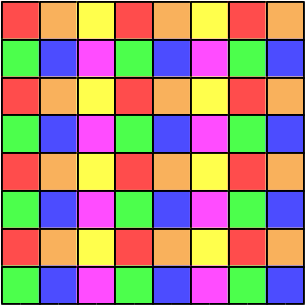
\includegraphics[scale=0.5]{scalapack.png}
\end{center}
\end{frame}

\begin{frame}{DAGuE}
\begin{exampleblock}{Advantages :}
\begin{itemize}
\item Independence between performances and computers
\item Provide multicore parallelism
\item Good reactivity for \textit{load in balance}
\item Natural look ahead
\end{itemize}
\end{exampleblock}{}
\pause
\begin{exampleblock}{Problems :}
\begin{itemize}
\item DAG is a static representation of a task flow
\end{itemize}
\end{exampleblock}{}
\end{frame}

